\documentclass[11pt]{article}

\author{Math 123}
\date{Due March 3, 2023 by \emph{midnight} } 
\title{Homework 5}

\usepackage{graphicx,xypic}
\usepackage{amsthm}
\usepackage{amsmath,amssymb}
\usepackage{amsfonts}
\usepackage{xcolor}
\usepackage[margin=1in]{geometry}
\usepackage[shortlabels]{enumitem}
\newtheorem{problem}{Problem}
\renewcommand*{\proofname}{{\color{blue}Solution}}


\usepackage{fancyhdr}
\pagestyle{fancy}
\rhead{Math 123, Homework 5}

\setlength{\parindent}{0pt}
\setlength{\parskip}{1.25ex}


\begin{document}

\maketitle

% You are required to put your name here:
{\bf\Large Name:} 


\vspace{.3in}
Topics covered: matchings, K\"onig's theorem, vertex covers, Gale--Shapely algorithm 

Instructions: 
\begin{itemize}
\item This assignment must be submitted on Gradescope by the due date. 
\item If you collaborate with other students (which is encouraged!), please mention this somewhere on the assignment. 
\item If you are stuck, please ask for help (from me, a TA, a classmate). Use Campuswire!  
\item You may freely use any fact proved in class. In general, you should provide proof for facts used that were not proved in class. 
\item {\bf Please restrict your solution to each problem to a single page.} Usually solutions can be even shorter than that. If your solution is very long, you should think more about how to express it concisely.
\end{itemize}

\pagebreak 



\begin{problem}
Let $G=(V,E)$ be a bipartite graph with maximum vertex degree $\Delta$. \begin{enumerate}[(a)]
\item Use K\"onig's theorem to prove that $G$ has a matching of size at least $|E|/\Delta$. 
\item Use (a) to conclude that every subgraph of $K_{n,n}$ with more than $(k-1)n$ edges has a matching of size at least $k$. 
\end{enumerate} 
\end{problem}

\begin{proof}

\end{proof}

\pagebreak



\begin{problem}
Fix $k\ge2$, and let $Q_k$ denote hypercube graph (from HW1). Prove that $Q_k$ has at least $2^{2^{k-2}}$ perfect matchings.
\end{problem}

\begin{proof}

\end{proof}

\pagebreak



\begin{problem}
Determine the stable matchings resulting from the proposal algorithm run with cats proposing and with giraffes proposing, given the preference lists below.
\begin{center}
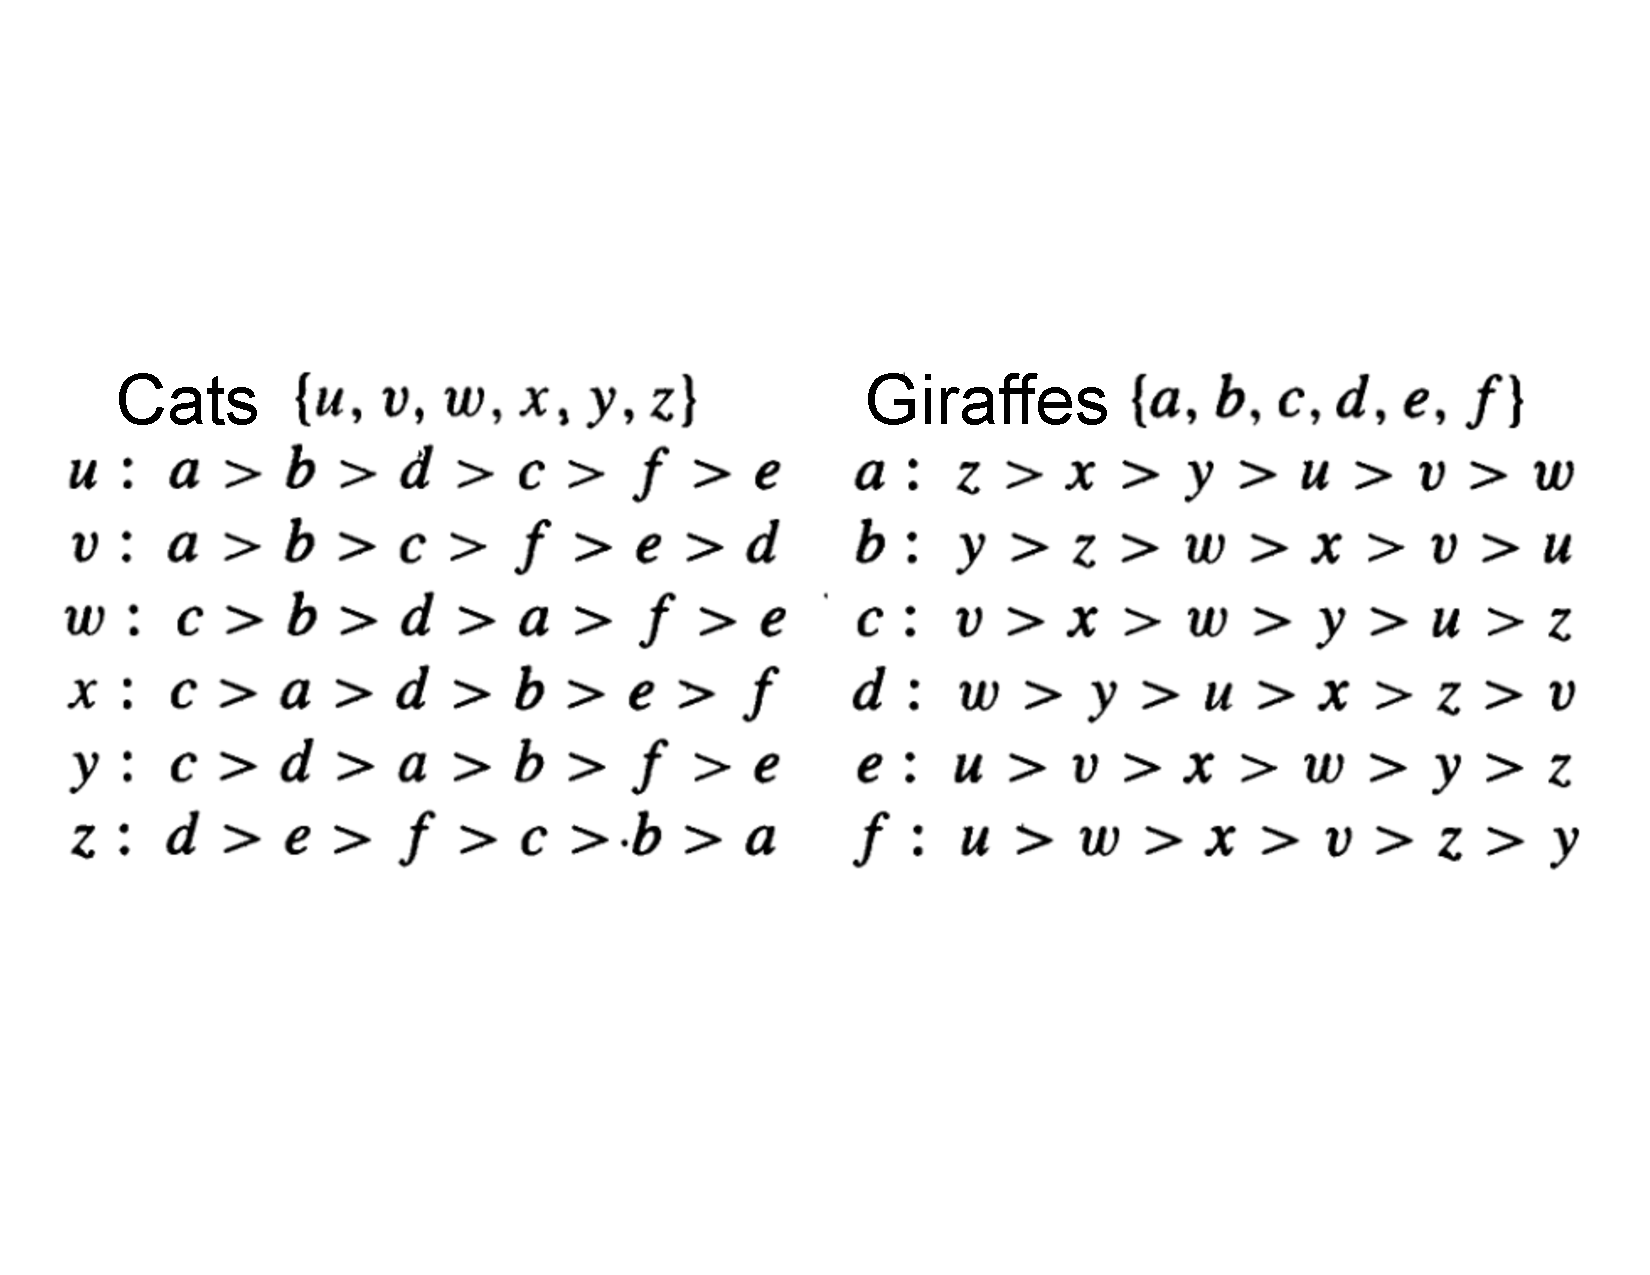
\includegraphics[scale=.5]{stable-match.pdf}
\end{center}
To receive full credit, you should show your work.
\end{problem}

\begin{proof}

\end{proof}

\pagebreak

\begin{problem}
Let $G=(X\sqcup Y,E)$ be a bipartite graph satisfying $|N(S)|>|S|$ for each nonempty $S\subset X$. Prove that every edge of $G$ belongs to some matching that saturates $X$. 
\end{problem}

\begin{proof}

\end{proof}

\pagebreak 

\begin{problem}
Complete the proof of K\"onig's theorem that we started in class. 
\end{problem}

\begin{proof}

\end{proof}

\pagebreak
\begin{problem}
A deck with $mn$ cards with $m$ values and $n$ suits consists of one card for each value in each suit. The cards are dealt into an $n\times m$ array. Prove that there is a set of $m$ cards, one in each column, having distinct values. 
\end{problem}

\begin{proof}

\end{proof}

\pagebreak


\pagebreak

\begin{problem}[Bonus]
Let $T_1$ be the tiling of the plane by unit squares whose vertices have integer coordinates. Let $T_2$ be the result of rotating $T_1$ about the origin by some angle $\theta$. Prove that it is possible to find a bijection between squares of $T_1$ and squares of $T_2$ in such a way that the matched squares are within 10 units of each other. The matching will depend on $\theta$. 
\end{problem}


\begin{proof}

\end{proof}


\end{document}